\documentclass[UTF8,AutoFakeBold]{ctexbook}
\usepackage{ctex}
\usepackage{framed}
\usepackage{amsthm}
\usepackage{geometry}
\usepackage{amsthm,amsmath,amssymb}
\usepackage{mathrsfs}
\geometry{left=2.0cm,right=2.0cm,top=2.0cm,bottom=2.0cm}
\usepackage{amsmath}
\usepackage{graphicx}
\usepackage{subfiles}
\usepackage{color}
\title{\kaishu\textbf {分析学}}
\author{\kaishu 张博涵(xb782053@gmail.com)\\
\kaishu bilibili:天才我张主教\\
\kaishu 知乎:小张也要开心}
\date{\kaishu \today}
\setCJKsansfont{KaiTi}
\usepackage{chemfig}
\usepackage{listings}
\usepackage{framed}
\usepackage{amsthm,amsmath,amssymb}
\usepackage{wrapfig}
\usepackage{graphicx}
\usepackage{mathrsfs}
\bibliographystyle{plain}
\usepackage{subfiles}
\usepackage{booktabs}
\usepackage{graphicx,times}
\usepackage{times}
\usepackage{subfigure}         
\usepackage{natbib}
\usepackage{amssymb,amsmath}
\usepackage{url}
\usepackage{geometry}
\usepackage{xcolor}
\usepackage{setspace}
\usepackage{subfigure}
\usepackage{tikz}
\everymath{\displaystyle}
\usepackage{booktabs}
\usepackage{array}
\usepackage{mhchem}
%\usepackage[usenames,dvipsnames]{color}
\usepackage{colortbl}


\definecolor{mygray}{gray}{.9}
\definecolor{mypink}{rgb}{.99,.91,.95}
\definecolor{mycyan}{cmyk}{.3,0,0,0}
\definecolor{myorgn}{rgb}{0.56,0.28,0.16}
\definecolor{myyelo}{rgb}{255,215,0}


\usepackage[breaklinks,colorlinks,linkcolor=black,citecolor=black,urlcolor=black]{hyperref}

\begin{document}

\begin{table}
    \centering
     \begin{tabular}{p{2cm}<{\centering} p{2cm}<{\centering} p{2cm}<{\centering} p{2cm}<{\centering} p{2cm}<{\centering} p{2cm}<{\centering}}
		\toprule
        $V$/mL & pH & $\Delta V$/mL & $\Delta$pH & $\dfrac{\Delta \ce{pH}}{\Delta V}$ & $\dfrac{\Delta^{2} \ce{pH}}{\Delta V^{2}}$ \\
        \midrule
        0.00 & 3.18 &  &  &  &  \\ 
        3.00 & 4.18 & 3.00 & 1.00 & 0.33 &  \\ 
        5.00 & 4.50 & 2.00 & 0.32 & 0.16 & -0.09  \\ 
        7.00 & 4.77 & 2.00 & 0.27 & 0.14 & -0.01  \\ 
        9.00 & 5.07 & 2.00 & 0.30 & 0.15 & 0.01  \\
        10.00 & 5.27 & 1.00 & 0.20 & 0.20 & 0.05  \\
        11.00 & 5.51 & 1.00 & 0.24 & 0.24 & 0.04  \\ 
        12.00 & 5.96 & 1.00 & 0.45 & 0.45 & 0.21  \\ 
        12.10 & 6.08 & 0.10 & 0.12 & 1.20 & 7.50  \\ 
        12.20 & 6.16 & 0.10 & 0.08 & 0.80 & -4.00  \\ 
        12.30 & 6.25 & 0.10 & 0.09 & 0.90 & 1.00  \\ 
        12.40 & 6.40 & 0.10 & 0.15 & 1.50 & 6.00  \\ 
        12.50 & 6.53 & 0.10 & 0.13 & 1.30 & -2.00  \\ 
        12.60 & 6.70 & 0.10 & 0.17 & 1.70 & 4.00  \\
        12.70 & 7.09 & 0.10 & 0.39 & 3.90 & 22.00  \\
        12.80 & 7.76 & 0.10 & 0.67 & 6.70 & 28.00  \\
        12.90 & 9.37 & 0.10 & 1.61 & 16.10 & 94.00  \\ 
        13.00 & 9.97 & 0.10 & 0.60 & 6.00 & -101.00  \\ 
        13.10 & 10.25 & 0.10 & 0.28 & 2.80 & -32.00  \\ 
        13.20 & 10.42 & 0.10 & 0.17 & 1.70 & -11.00  \\
        13.30 & 10.62 & 0.10 & 0.20 & 2.00 & 3.00  \\ 
        13.40 & 10.76 & 0.10 & 0.14 & 1.40 & -6.00  \\ 
        13.50 & 10.87 & 0.10 & 0.11 & 1.10 & -3.00  \\ 
        13.60 & 10.94 & 0.10 & 0.07 & 0.70 & -4.00  \\ 
        13.70 & 11.04 & 0.10 & 0.10 & 1.00 & 3.00  \\ 
        14.70 & 11.47 & 1.00 & 0.43 & 0.43 & -0.57  \\ 
        15.70 & 11.70 & 1.00 & 0.23 & 0.23 & -0.20  \\ 
        16.70 & 11.84 & 1.00 & 0.14 & 0.14 & -0.09  \\ 
        18.70 & 12.02 & 2.00 & 0.18 & 0.09 & -0.03  \\ 
        20.70 & 12.14 & 2.00 & 0.12 & 0.06 & -0.01  \\ 
        22.70 & 12.23 & 2.00 & 0.09 & 0.04 & -0.01  \\        \bottomrule
    \end{tabular}
    \caption{具体数据处理数值}
\end{table}

\begin{figure}[h]
 	\centering
	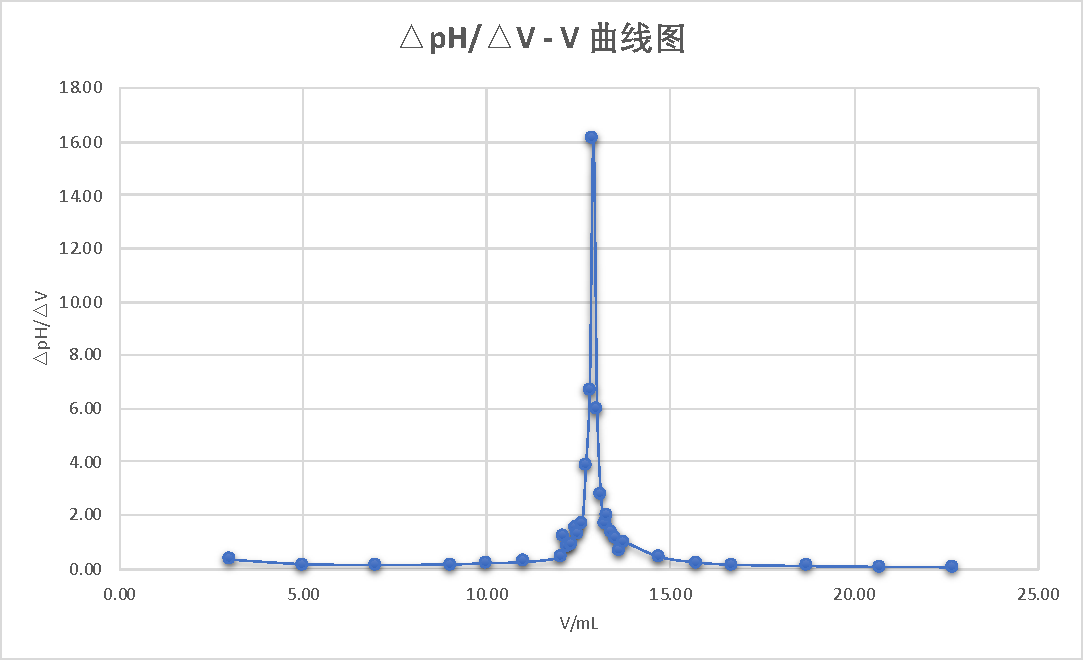
\includegraphics[scale=0.7]{一阶微商图}
 \end{figure}
 \begin{figure}[h]
 	\centering
	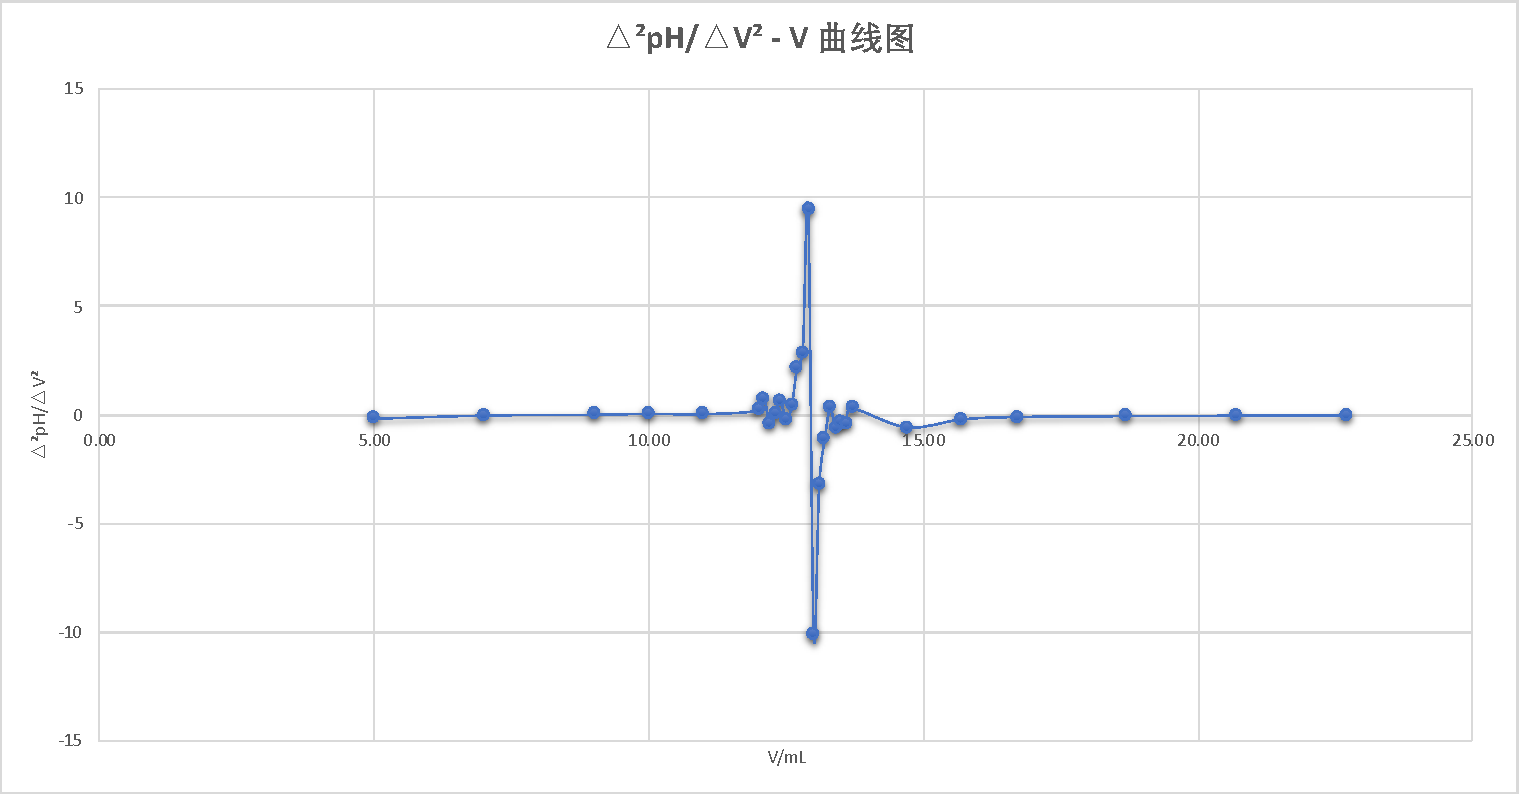
\includegraphics[scale=0.7]{二阶微商图}
 \end{figure}
 \begin{figure}[h]
 	\centering
	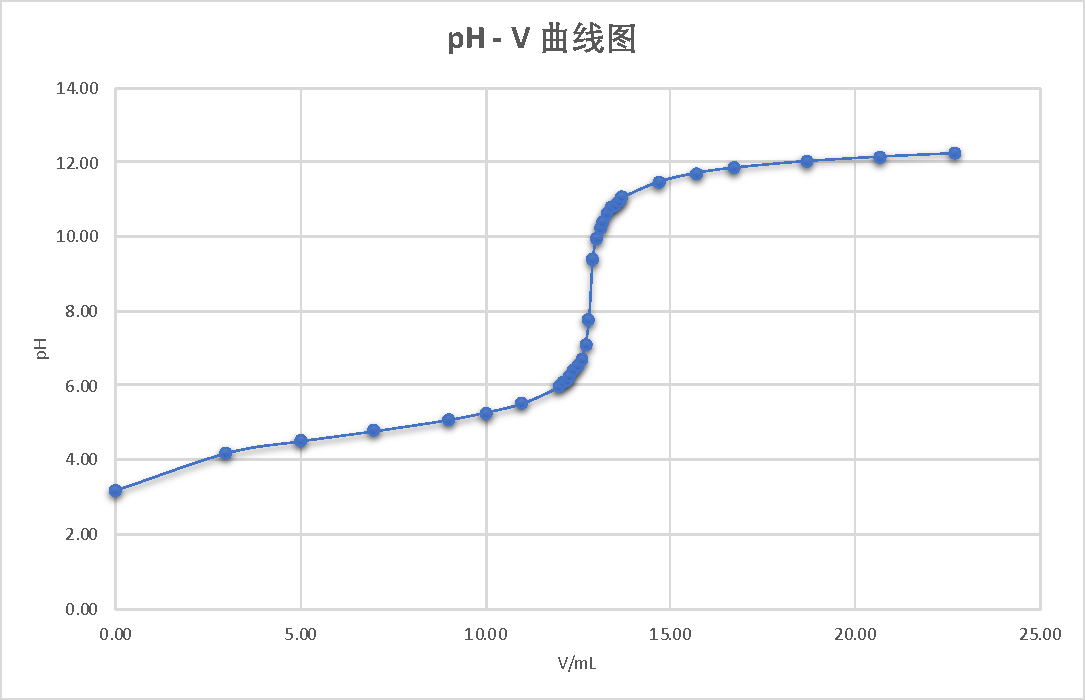
\includegraphics[scale=0.7]{曲线图}
 \end{figure}

\end{document}